% article_FR_5.0.tex — one-page presentation of WAC 5.0 for a DFIR magazine,
% French edition. The English edition is article_EN_5.0.tex, in this folder:
% both are maintained together, paragraph for paragraph. It follows the article
% on version 4.0 (article_FR_4.0.tex) and presents only what 5.0 adds.
%
% Build (LuaLaTeX, as the editor's recipe; build artefacts removed after):
%     ../build-docs.sh article/article_FR_5.0.tex
%
% Every figure comes from the validation and harmlessness files
% (doc/validation, doc/harmlessness) and the backlog, measured from 8 to
% 13 November 2026 on the code of 5.0. Backlog B-075.

\documentclass[10pt,a4paper,twocolumn]{article}
\usepackage[french]{babel}
\usepackage{fontspec}
\setmainfont{Noto Sans}
\setmonofont{DejaVu Sans Mono}[Scale=0.84]
\usepackage[top=13mm,bottom=13mm,left=14mm,right=14mm,columnsep=7mm]{geometry}
\usepackage{xcolor}
\usepackage{titlesec}
\usepackage{enumitem}
\usepackage{array}
\usepackage{graphicx}
\usepackage{caption}
\captionsetup{font={small,color=gris},skip=2pt}
\usepackage[hidelinks]{hyperref}
\definecolor{marine}{HTML}{0A1A33}
\definecolor{bleu}{HTML}{2F6DB5}
\definecolor{gris}{HTML}{5B6573}
\pagestyle{empty}
\setlength{\parindent}{0pt}
\setlength{\parskip}{0.35em}
\titleformat{\section}{\color{marine}\normalsize\bfseries}{}{0em}{}
\titlespacing*{\section}{0pt}{0.7em}{0.2em}
\setlist{nosep,leftmargin=1.1em}
\newcommand{\wac}{\textsc{wac}}
\newcommand{\fichier}[1]{\texttt{#1}}
\hypersetup{pdftitle={WAC 5.0 — les traces des applications, datées juste}}

\begin{document}

\twocolumn[{%
  {\color{marine}\LARGE\bfseries WAC 5.0 : les traces des applications, datées juste}\par
  \vspace{0.3em}
  {\color{gris}Centre d'Excellence Cyberdéfense Aérospatiale (CEC), École de l'air et de l'espace}\par
  \vspace{0.6em}
  {\itshape \wac{} (Windows Artefacts Collector) est un collecteur libre, en
  C++, qui lit les volumes en brut sans rien écrire sur la machine examinée, des
  postes XP~SP1 à Windows~11 et des serveurs 2003 à 2025. La version 5.0 prend
  ce que les applications gardent hors des journaux d'événements, et date
  chaque heure écrite sans fuseau avec le fuseau en vigueur quand elle a été
  écrite.}\par
  \vspace{0.9em}
}]

\section{97 produits, une table}
Outils d'administration à distance (TeamViewer, AnyDesk, RustDesk,
ScreenConnect\ldots), antivirus autres que Defender, messageries, stockage en
ligne, transfert de fichiers, VPN, virtualisation, applications et journaux de
serveur (Netlogon, NPS, autorité de certification), et ce que Windows garde en
plus : 97 produits en onze groupes, chacun avec ses dossiers, la plupart tirés
des cibles de KAPE, et son interrupteur dans \fichier{wac.yml}. PuTTY, WinSCP,
WinRAR et 7-Zip sont lus dans la ruche de chaque utilisateur. Les dossiers sont
lus en brut, comme le reste : rien n'est ouvert par le système.

\section{Copiés, puis convertis}
KAPE copie ces fichiers ; \wac{} les copie et les convertit, sans un décodeur
par produit : un journal devient un élément par ligne, avec la date qui
l'ouvre ; XML, JSON et INI donnent leur structure ; une base ou un binaire est
listé et reste dans la consigne. Une valeur nommée comme un mot de passe, un
bloc de clé privée d'un profil OpenVPN, ne sont jamais écrits : le JSON dit
seulement qu'ils existent. Les clés privées SSH ne sont pas prises ; les
vidages de plantage et le cache d'Office, qui peuvent porter des documents,
sont coupés par défaut.

\section{L'heure écrite sans fuseau}
Une heure d'horloge n'est pas un instant. \wac{} la convertit avec le fuseau en
vigueur quand elle a été écrite, tiré du journal Système : chaque changement de
décalage depuis Windows~10, le fuseau observé au démarrage et chaque jour
avant. Un changement dont aucun événement ne donne l'instant reste un
intervalle, jamais un instant inventé ; une heure vécue deux fois donne ses
autres instants possibles. Pour chaque produit présent dans les machines de
test, le fuseau supposé a été mesuré contre l'horloge : une ligne provoquée,
encadrée par l'heure système. TeamViewer, une ligne écrite sous un autre
fuseau, l'heure répétée d'octobre : datés à la milliseconde, comme Windows les
convertit.

\section{Ce que la revue a trouvé}
La revue de code et de sécurité de la 5.0 a corrigé deux défauts avant la
publication : une clé privée d'un fichier texte serait sortie en clair dans le
JSON, et un index NTFS forgé, nommant un dossier comme son propre motif,
faisait boucler la collecte jusqu'au débordement de pile. Chacun a son test,
vu échouer avant le correctif ; les lecteurs de la 5.0 passent 46\,000 entrées
mutées sans lecture hors tampon.

\section{Ce qui reste à mesurer}
Un témoin prouve que le chemin de la table est pris, pas que chaque version
d'un produit écrit là : la plupart des 97 produits n'étaient pas installés
dans les machines de test, et leur heure est supposée locale sans
vérification. UltraViewer écrit sa date dans le format de la culture du
compte : elle n'est pas lue. La comparaison mesurée face à KAPE reste celle du
29 octobre, antérieure à ces cibles.

\section{En chiffres}
\begin{tabular}{@{}>{\raggedright\arraybackslash}p{0.75\columnwidth}@{\hspace{0.5em}}r@{}}
Artefacts prélevés (4.0 : 87) & 99 \\
Produits de la table des traces & 97 \\
Contrôles du cycle, Windows~11 & 677 \\
Entrées mutées, lecteurs de la 5.0 & 46\,000 \\
Mots de passe ou clés privées écrits & 0 \\
\end{tabular}

\section{Disponibilité}
Version 5.0.0, Windows~XP~SP1 à 11 et Server~2003 à 2025 (x86 et x64), licence
GPL~3.0 : \url{https://github.com/dev-cec/WAC}. Manuels, dossiers de validation,
d'innocuité et de comparaison en français et en anglais ; cycles du 8 au
13 novembre 2026.

\vfill
\begin{center}
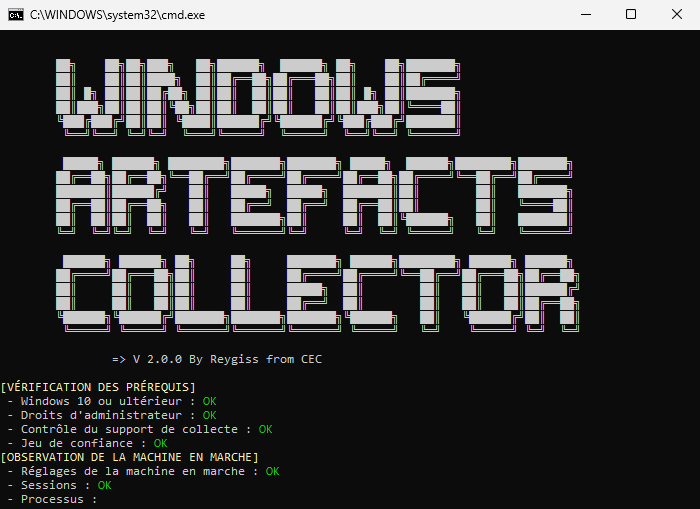
\includegraphics[width=\columnwidth,height=24mm,keepaspectratio]{../images/wac-running_FR.png}
\captionof*{figure}{\wac{} en cours de collecte.}
\end{center}

\end{document}
